\documentclass[12pt, oneside, openany]{article}
\usepackage[T1]{fontenc}
\usepackage[spanish, es-tabla, es-lcroman]{babel}
\usepackage[utf8]{inputenc}
\usepackage[document]{ragged2e}
\usepackage{tcolorbox}
\tcbuselibrary{theorems}
\usepackage{cancel}
\usepackage{amssymb}
\usepackage{amsmath}
\usepackage{mathrsfs}
\usepackage{wrapfig}
\usepackage{fancyhdr}
\usepackage{colortbl}
\usepackage{graphicx}
\usepackage{subcaption}
\usepackage{xcolor}
\usepackage{tikz}
\usepackage{multicol}
\usepackage{multirow}
\usepackage{lastpage}
\usepackage{pdfpages}
\usepackage{listings}
\usepackage{blindtext}
\spanishdecimal{.}
\usepackage[explicit]{titlesec}
\usepackage[colorlinks=true, linkcolor=black, citecolor=black, urlcolor=blue]{hyperref}
\usepackage[a4paper, total={16cm, 24cm}]{geometry}
\pagestyle{fancy}
\lhead{Muñoz Nuñez Ian Emmanuel}
\rhead{Proyecto 1}
\lfoot{Mtra. Maria Patricia Ventura Nuñez}
\rfoot{CUCEI}
\renewcommand{\headrulewidth}{1pt}
\renewcommand{\footrulewidth}{1pt}
\renewcommand{\labelitemi}{$\bullet$}

\begin{document}

\begin{titlepage}
    \pagenumbering{roman}
    \centering
    {\bfseries\LARGE Universidad de Guadalajara \par}
    \vfill
    {\bfseries\LARGE Centro Universitario de Ciencias Exactas e Ingenierías (CUCEI) \par}
    \vfill
    {
        \includegraphics[width=0.3\linewidth]{UdG.png}
        \includegraphics[width=0.3\linewidth]{qci.png}
        \par
    }
    \vfill
    {\bfseries\LARGE Seminario de Problemas de Programación de Sistemas Reconfigurables \par}
    \vfill
    {\bfseries\LARGE Proyecto 1 \par}
    \vfill
    {\LARGE Implementación de un circuito lógico combinacional utilizando compuertas lógicas básicas (and, or, not) \par}
    \vfill
    {\bfseries\LARGE Nombre: \par}
    \vfill
    {\bfseries\LARGE Muñoz Nuñez Ian Emmanuel \par}
    \vfill
    {\bfseries\LARGE Sección: D01 \par}
    \vfill
    {\bfseries\LARGE Código: 216464457 \par}
    \vfill
    {\bfseries\LARGE Maestra: \par}
    \vfill
    {\bfseries\LARGE María Patricia Ventura Nuñez \par}
    \vfill
    {\bfseries\LARGE Ingeniería Robótica \par}
\end{titlepage}

\pagenumbering{arabic}
\newpage
\section{Objetivo}
{\sffamily\Large
    \hspace{0.5cm} Solucionar problemas de diseño utilizando las herramientas aprendidas en Programación de Sistemas Reconfigurables.
    
    \hspace{0.5cm} Utilizar hojas de datos de las familias lógicas.
    
    \hspace{0.5cm} Simular circuitos digitales en programas de diseño como \emph{Proteus\texttrademark} e implementarlos físicamente.
    
    \hspace{0.5cm} Comprender el funcionamiento de las compuertas lógicas básicas (\emph{and}, \emph{or}, \emph{not}).
    
}

\section{Material}
{\sffamily\Large
    \begin{itemize}
        \item Protoboard.
        \item Fuente Vcc (5V).
        \item Led.
        \item Resistencias de 200$\Omega$ y 2$k\Omega$.
        \item 1 dip switch de 8 bits.
        \item 1 74LS04 $\to$ inversor o compuerta lógica \emph{not}.
        \item 2 74LS08 $\to$ compuerta lógica \emph{and} de 2 entradas.
        \item 1 74LS32 $\to$ compuerta lógica \emph{or} de 2 entradas.
    \end{itemize}
    
}

\section{Marco teórico}
{\sffamily\Large
    \hspace{0.5cm} Diseñar un circuito combinacional para la siguiente función de \emph{ABCDE} donde:
    F(A, B, C, D, E)=1 cuando ABD entre CE = Número impar
    
    \hspace{0.5cm} NOTA:
    \begin{itemize}
        \item Cuando el resultado sea indeterminado o tenga fracción será igual a 0.
        \newpage
        \item Cuando el resultado de la división sea 0 será considerado como par.
    \end{itemize}
    
    \begin{table}[h!]
        \centering
        \sffamily
        \begin{tabular}{|c|c|c|c|c|c|c|}
            \hline
            & A & B & C & D & E & F\\
            \hline
            0  & 0 & 0 & 0 & 0 & 0 & 0\\
            \hline
            1  & 0 & 0 & 0 & 0 & 1 & 0\\
            \hline
            2  & 0 & 0 & 0 & 1 & 0 & 0\\
            \hline
            3  & 0 & 0 & 0 & 1 & 1 & 1\\
            \hline
            4  & 0 & 0 & 1 & 0 & 0 & 0\\
            \hline
            5  & 0 & 0 & 1 & 0 & 1 & 0\\
            \hline
            6  & 0 & 0 & 1 & 1 & 0 & 0\\
            \hline
            7  & 0 & 0 & 1 & 1 & 1 & 0\\
            \hline
            8  & 0 & 1 & 0 & 0 & 0 & 0\\
            \hline
            9  & 0 & 1 & 0 & 0 & 1 & 0\\
            \hline
            10 & 0 & 1 & 0 & 1 & 0 & 0\\
            \hline
            11 & 0 & 1 & 0 & 1 & 1 & 1\\
            \hline
            12 & 0 & 1 & 1 & 0 & 0 & 1\\
            \hline
            13 & 0 & 1 & 1 & 0 & 1 & 0\\
            \hline
            14 & 0 & 1 & 1 & 1 & 0 & 0\\
            \hline
            15 & 0 & 1 & 1 & 1 & 1 & 1\\
            \hline
            16 & 1 & 0 & 0 & 0 & 0 & 0\\
            \hline
            17 & 1 & 0 & 0 & 0 & 1 & 0\\
            \hline
            18 & 1 & 0 & 0 & 1 & 0 & 0\\
            \hline
            19 & 1 & 0 & 0 & 1 & 1 & 1\\
            \hline
            20 & 1 & 0 & 1 & 0 & 0 & 0\\
            \hline
            21 & 1 & 0 & 1 & 0 & 1 & 0\\
            \hline
            22 & 1 & 0 & 1 & 1 & 0 & 0\\
            \hline
            23 & 1 & 0 & 1 & 1 & 1 & 0\\
            \hline
            24 & 1 & 1 & 0 & 0 & 0 & 0\\
            \hline
            25 & 1 & 1 & 0 & 0 & 1 & 0\\
            \hline
            26 & 1 & 1 & 0 & 1 & 0 & 0\\
            \hline
            27 & 1 & 1 & 0 & 1 & 1 & 1\\
            \hline
            28 & 1 & 1 & 1 & 0 & 0 & 0\\
            \hline
            29 & 1 & 1 & 1 & 0 & 1 & 0\\
            \hline
            30 & 1 & 1 & 1 & 1 & 0 & 0\\
            \hline
            31 & 1 & 1 & 1 & 1 & 1 & 0\\
            \hline
        \end{tabular}
        \caption{\sffamily Tabla de verdad}
        \label{tab:tablaVerdad}
    \end{table}
    
}

\newpage
\section{Procedimiento}
{\sffamily\Large
    \hspace{0.5cm} Implementación de un circuito lógico combinacional utilizando compuertas lógicas básicas (and, or, not).
    
    \hspace{0.5cm} Para realizar el proyecto se debe tener cuidado al realizar las conexiones con cada una de las compuertas, pues tener mal una conexión implica tener resultados no deseados. Además, se debe probar cada componente a usar para saber que todo se encuentre en buenas condiciones, pues sí un componente está dañado, nos puede dar problemas al momento de implementar nuestro circuito.
    
    \hspace{0.5cm} Una vez que estemos seguros de que todos los componentes están en óptimas condiciones y el circuito está bien conectado, alimentamos este y probamos las operaciones de la tabla de verdad.
    
    \hspace{0.5cm} Los materiales que se utilizaron para esta práctica son: 1 dip switch de 8 bits, 1 led, 1 resistencia de 220$\Omega$ y 5 resistencias de 2$k\Omega$, 1 inversor o compuerta \emph{not}, 2 compuertas \emph{and} y una compuerta \emph{or}.
    
}

\section{Simulación}
{\sffamily\Large
    \hspace{0.5cm} Las conexiones realizadas se muestran en la siguiente imagen.
    \begin{figure}[h!]
        \centering
        \includegraphics[width=0.7\linewidth]{proteus.png}
        \caption{\sffamily Simulación relizada en \emph{Proteus\texttrademark}}
        \label{fig:simulacion}
    \end{figure}
    
}

\newpage
\section{Protoboard}
{\sffamily\Large
    \hspace{0.5cm} El resultado de la práctica se muestra a continuación.
    \begin{figure}[h!]
        \centering
        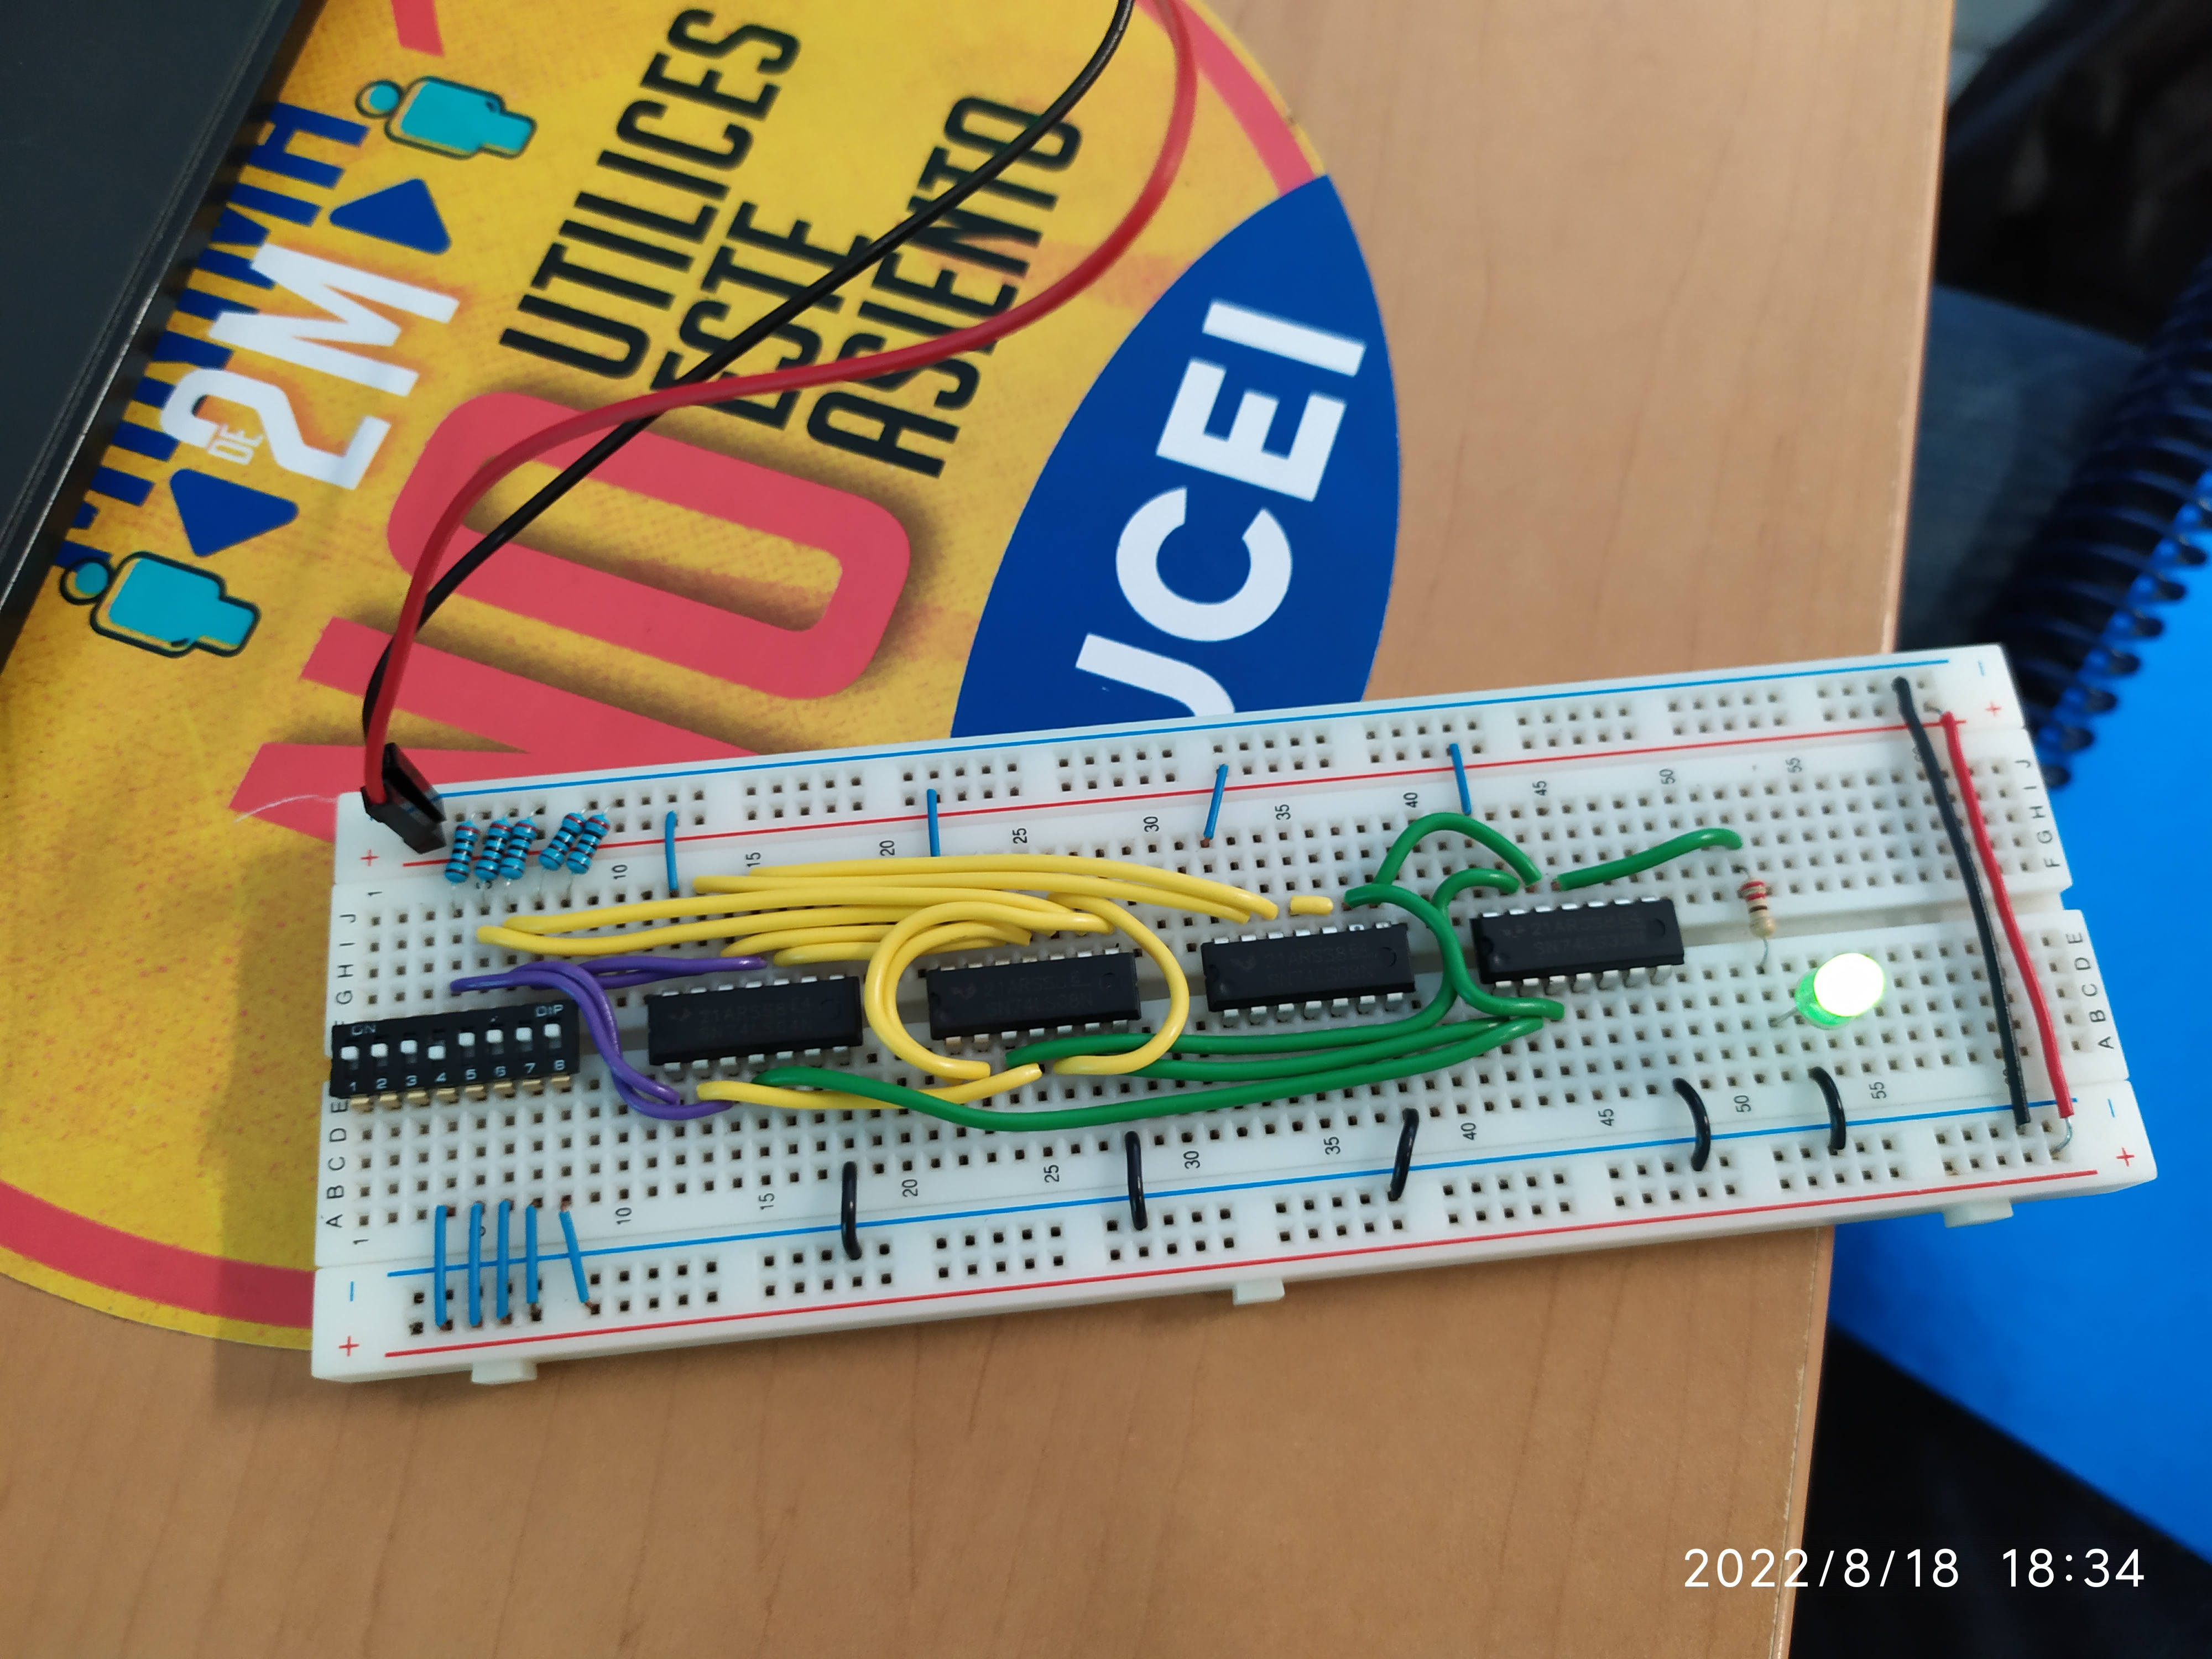
\includegraphics[width=0.7\linewidth]{proto1.jpg}
        \caption{\sffamily Circuito en Protoboard}
        \label{fig:proto}
    \end{figure}
    
}

\section{Conclusión}
{\sffamily\Large
    \hspace{0.5cm} Es muy interesante conocer el funcionamiento de las compuertas lógicas, pues son una de las bases de todo dispositivo electrónico, y creo que es importante conocer por lo menos un poco sobre el funcionamiento de un circuito lógico.
    
    \hspace{0.5cm} Me gusto mucho hacer este proyecto, pues no sabia nada sobre como hacer un circuito lógico. Una de las partes que más se me complicó fue poner atención de en donde conectaba las entradas y las salidas de cada compuerta, pues al haber tantos cables me confundía.
    
}

\end{document}
